\documentclass[12pt,a4paper]{article}

% --- Packages ---
\usepackage[utf8]{inputenc}
\usepackage[T1]{fontenc}
\usepackage{geometry}
\usepackage{graphicx}
\usepackage{hyperref}
\usepackage{titlesec}
\usepackage{setspace}
\usepackage{listings}
\usepackage{xcolor}
\usepackage{float} 
\usepackage{tikz}
\usetikzlibrary{shapes,arrows,positioning,shadows}

% --- Page Setup ---
\geometry{margin=1in}
\onehalfspacing

% --- Custom colors for code listings ---
\definecolor{codegray}{rgb}{0.5,0.5,0.5}
\definecolor{codeblue}{rgb}{0.0,0.0,0.8}
\definecolor{codegreen}{rgb}{0,0.6,0}

\lstset{
    backgroundcolor=\color{white},
    commentstyle=\color{codegreen},
    keywordstyle=\color{codeblue},
    numberstyle=\tiny\color{codegray},
    stringstyle=\color{red},
    basicstyle=\ttfamily\small,
    breakatwhitespace=false,
    breaklines=true,
    captionpos=b,
    keepspaces=true,
    numbers=left,
    numbersep=5pt,
    showspaces=false,
    showstringspaces=false,
    showtabs=false,
    tabsize=2
}

\begin{document}

% --- TITLE PAGE ---
\begin{titlepage}
    \centering
    \vspace*{2cm}
    
\includegraphics[width=0.4\textwidth]{icon1.png} 
    \vspace{1.5cm}
    
    {\Huge \textbf{ChatTalk} \par}
    \vspace{0.5cm}
    {\Large \textit{The Ultimate Real-time Messaging Ecosystem} \par}
    
    \vspace{2cm}
    {\large \textbf{Project Report} \par}
    \vspace{1cm}
    
    {\large Submitted by \par}
    {\Large \textbf{Ankush Verma} \par}
    
    \vfill

\end{titlepage}

% --- FRONT MATTER (Abstract & TOC) ---
\newpage
\pagenumbering{roman}

\begin{abstract}
ChatTalk is a powerful, high-performance messaging application developed using the MERN (MongoDB, Express, React, Node.js) stack. It is designed to provide a seamless, modern, and highly interactive chat experience for users. By leveraging event-driven architecture with Socket.io, ChatTalk achieves real-time synchronization of messages, typing indicators, read receipts, and user status across all connected platforms. The core database infrastructure rests on Mongoose schemas handling User, Chat, Message, and Friend Request modules securely. This report provides a comprehensive overview of the application's robust architecture, intricate feature implementations, technology stack, and extensive security measures utilizing JWT-in-Cookie patterns and Bcrypt encryption.
\end{abstract}
\newpage

\tableofcontents
\newpage

% --- MAIN CONTENT ---
\pagenumbering{arabic}
\setcounter{page}{1}

\section{Introduction}

\subsection{Project Overview}
\textbf{ChatTalk} is a full-stack real-time messaging application engineered to ensure users have a secure and lightning-fast platform for communication. Integrating cutting-edge frontend technologies like React and Material UI with an industrial-grade Node.js and Express backend, it establishes a unified WebSocket layer for instant communication. The application is modular, incorporating a centralized API server, a highly responsive Single Page Application (SPA), and a real-time event broadcaster.

\subsection{Problem Statement}
Modern digital communication demands low latency, absolute security, and an intuitive user interface. Traditional HTTP-based chat applications are inadequate, often plagued by message delivery delays, polling overhead, and fragmented authentication flows. ChatTalk aims to solve these prevailing issues by implementing a unified real-time duplex data stream with an optimized MongoDB database architecture and strict cross-domain stable JWT-based authentication.

\subsection{Objectives}
\begin{itemize}
    \item \textbf{Low-Latency Real-Time Ecosystem}: Develop a high-performance system capable of instant messaging, active typing indicators, and reliable delivery statuses.
    \item \textbf{Comprehensive Schema Infrastructure}: Manage entities securely via distinct logical modules for Users, Messages, Chats (1-to-1 \& Groups), and Friend Requests.
    \item \textbf{Advanced Security Constraints}: Implement fortified authentication leveraging bcrypt password hashing alongside HttpOnly secured cookies holding JSON Web Tokens (JWT).
    \item \textbf{Media \& Attachments Engine}: Enable rich media sharing directly within chat windows powered by the Cloudinary API.
    \item \textbf{Actionable Admin Dashboard}: Facilitate platform moderation, statistical overviews, and system analytics through a dedicated administrative portal.
\end{itemize}

\section{System Architecture}

\subsection{High-Level Design}
ChatTalk operates as a \textbf{Unified Real-time Distributed System} operating precisely across three core functional layers:
\begin{enumerate}
    \item \textbf{Frontend Presentation Layer}: A dynamic React-based SPA that robustly manages user interface components, reactive state pooling via Redux Toolkit, and handles UX responsiveness.
    \item \textbf{Backend REST API Layer}: A Node.js and Express server handling resource routing, intricate business logic, model validations, and synchronous interactions with the database.
    \item \textbf{Real-time Synchronization Stream}: A dedicated, stateful WebSocket protocol layer powered by Socket.io, facilitating persistent bidirectional connections for sub-second data broadcasts.
\end{enumerate}

\subsection{Architecture Diagram}
\begin{center}
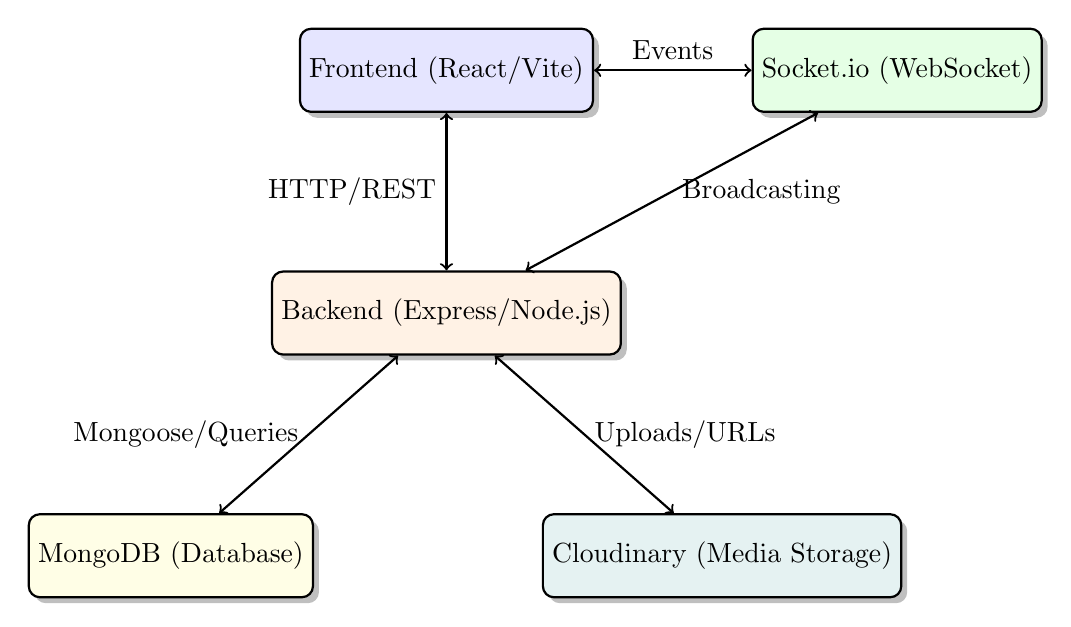
\begin{tikzpicture}[
    node distance=2cm, 
    style/.style={rectangle, draw=black, thick, fill=blue!10, text centered, rounded corners, minimum height=3em, minimum width=10em, drop shadow}
]
\node (client) [style] {Frontend (React/Vite)};
\node (socket) [style, right=of client, fill=green!10] {Socket.io (WebSocket)};
\node (server) [style, below=of client, fill=orange!10] {Backend (Express/Node.js)};
\node (db) [style, below=of server, xshift=-3.5cm, fill=yellow!10] {MongoDB (Database)};
\node (cloudinary) [style, below=of server, xshift=3.5cm, fill=teal!10] {Cloudinary (Media Storage)};

\draw[<->, thick] (client) -- node[above] {Events} (socket);
\draw[<->, thick] (client) -- node[left] {HTTP/REST} (server);
\draw[<->, thick] (server) -- node[left] {Mongoose/Queries} (db);
\draw[<->, thick] (server) -- node[right] {Uploads/URLs} (cloudinary);
\draw[<->, thick] (socket) -- node[right] {Broadcasting} (server);
\end{tikzpicture}
\end{center}

\subsection{Database Schema Design}
The foundation of ChatTalk relies on four distinct NoSQL schemas modeled using Mongoose:
\begin{itemize}
    \item \textbf{User Model}: Secures core identity, carrying encrypted passwords, avatars mapped to Cloudinary URLs, distinct usernames, biographies, and tracks `lastSeen` metadata for online presence.
    \item \textbf{Chat Model}: Determines context, distinguishing gracefully between individualized one-on-one relationships vs. multi-member group conversations, securely referencing the `User` instances who participate.
    \item \textbf{Message Model}: Stores granular conversational history, encompassing complex objects such as Cloudinary attachments, specific user reactions (emojis), nested replies, and current read status (\texttt{sent, delivered, seen}).
    \item \textbf{Request Model}: Manages asynchronous platform interactions, facilitating pending, accepted, or rejected multi-user interaction states (such as connection requests).
\end{itemize}

\subsection{Interaction Flow}
The real-time lifecycle of an outbound chat message exhibits an optimized flow:
\begin{enumerate}
    \item The client locally dispatches a \texttt{NEW\_MESSAGE} event over the active TCP/WebSocket connection concurrently while maintaining optimistic UI updates.
    \item The Node server intercepts the payload, rapidly authenticates the session, and triggers an insert query into the MongoDB \texttt{Message} collection. Any multipart file attachments are simultaneously tunneled to Cloudinary.
    \item The server identifies connected socket namespaces corresponding to the chat members.
    \item The updated message document is instantly broadcasted strictly to the targeted users' unique socket IDs.
    \item Recipient clients ingest the emission, subsequently firing Redux actions to flawlessly update their virtual DOM elements in real-time.
\end{enumerate}

\section{Technology Stack}

\subsection{Frontend Technologies}
\begin{itemize}
    \item \textbf{Core Framework}: React.js bootstrapped radically fast via Vite.
    \item \textbf{Design System}: Material UI (MUI) for standardized, accessible, and theme-able interface components.
    \item \textbf{State Architecture}: Redux Toolkit (RTK) coupled tightly with RTK Query for sophisticated caching, invalidation, and external API abstractions.
    \item \textbf{Responsive Motion}: Framer Motion executing hardware-accelerated fluid micro-interactions.
    \item \textbf{Real-Time Stream}: \texttt{socket.io-client} parsing web socket traffic.
    \item \textbf{Data Visualization}: Chart.js implemented strategically for administrative data rendering.
\end{itemize}

\subsection{Backend Operations}
\begin{itemize}
    \item \textbf{Compute Engine}: Node.js paired with Express.js to orchestrate asynchronous REST pipelines.
    \item \textbf{Database Persistence}: Native MongoDB leveraging Mongoose Object Data Modeling (ODM).
    \item \textbf{Remote File Management}: Cloudinary Node SDK to process optimized media ingestion and on-the-fly image transformations.
    \item \textbf{Authentication}: JSON Web Tokens (JWT) bound strictly within HttpOnly browser cookies.
    \item \textbf{Security \& Upload Middleware}: Multer for parsing \texttt{multipart/form-data}, Bcrypt for rigorous one-way cryptographic hashing of credentials, and Helmet.js/CORS mapping tight resource boundaries.
\end{itemize}

\section{Key Features \& Implementations}

\subsection{Comprehensive Real-Time Intelligence}
Beyond standard messaging, ChatTalk synchronizes vital humanizing nuances continuously. Active typing indicators bounce dynamically via \texttt{START\_TYPING} and \texttt{STOP\_TYPING} socket events. Additionally, read receipts track granular delivery states traversing from "sent" to "seen" populated within the message schema arrays.

\subsection{Robust Authentication Paradigm}
Employing an uncompromising strategy using a JWT-in-Cookie infrastructure guarantees secure authentication bypassing traditional XSS (Cross-Site Scripting) vulnerabilities associated with LocalStorage. Backed structurally by a \texttt{userSchema.pre("save", ...)} Mongoose middleware, passwords endure auto-hashing mechanisms prior to commit. Certain sophisticated adjustments inherently accommodate Apple device (Safari) partitioning policies.

\subsection{Complex Messaging Options: Multimedia, Reactions, \& Replies}
ChatTalk extends standard text communication drastically by equipping the message schema with polymorphic properties. Users can embed Cloudinary-hosted file payloads, apply inline emoji reactions directly targeted at specific messages, and orchestrate direct nested replies citing previous contexts, mirroring capabilities characteristic of industry-leading communicative engines.

\subsection{Granular Administrative Dashboard}
Developed as a siloed, fully protected domain strictly reserved for administrative profiles. The dashboard exposes aggregated platform health metrics directly extracted via complex Mongoose aggregation pipelines. It portrays interactive graphical metrics regarding platform activity, active connections, database size, and user moderation controls cleanly.

\section{Results and Technical Achievements}

\subsection{Project Directory \& Organizational Structure}
The architectural arrangement was modularized deliberately to enforce clean, maintainable scaling:
\begin{itemize}
    \item \texttt{client/src/}: Cultivates a global Redux store topology alongside isolated domain-specific UI components and hook abstractions.
    \item \texttt{server/}: Orchestrates strict separation of concerns across controllers, model definitions, socket emission handlers, and stringent security middlewares.
\end{itemize}

\subsection{Screenshots}
\begin{figure}[H]
    \centering
    % Ensure chat_interface.png exists or use placeholder logic
    \includegraphics[width=0.85\textwidth]{chat_interface.png}
    \caption{Real-time Chat Interface rendering dynamic Redux-bound views and live Socket connection.}
\end{figure}

\begin{figure}[H]
    \centering
    % Ensure admin_dashboard.png exists or use placeholder logic
    \includegraphics[width=0.85\textwidth]{admin_dashboard.png}
    \caption{Admin Dashboard showcasing Visual Analytics parsed via Mongoose Aggregations.}
\end{figure}

\section{Conclusion}
The ChatTalk deployment conclusively validates the immense capacity of the modern MERN stack coupled intrinsically with WebSockets. It successfully shifts abstract development tenets into a production-ready construct, underscoring advanced schema modeling, defensive backend configurations, responsive UI implementation, and millisecond-latency streaming.

\end{document}
